\documentclass[norsk]{article}
\usepackage{amsmath}
\usepackage[mathletters]{ucs}
\usepackage[utf8x]{inputenc}
\usepackage[norsk]{babel}
\usepackage{esint}
\usepackage{physics,amssymb}
% \usepackage{nath}
% \delimgrowth=1
\usepackage{graphicx}
\usepackage{xcolor}
\usepackage[colorlinks]{hyperref}
\usepackage{cleveref}
\usepackage{listings}
\usepackage{subfig}
\usepackage{booktabs}
\usepackage{caption}
\usepackage{listings}
\definecolor{codegreen}{rgb}{0,0.6,0}
\definecolor{codegray}{rgb}{0.5,0.5,0.5}
\definecolor{codepurple}{rgb}{0.58,0,0.82}
\definecolor{backcolour}{rgb}{0.95,0.95,0.92}
\lstdefinestyle{mystyle}{
    backgroundcolor=\color{backcolour},   
    commentstyle=\color{codegreen},
    keywordstyle=\color{magenta},
    numberstyle=\tiny\color{codegray},
    stringstyle=\color{codepurple},
    basicstyle=\ttfamily\footnotesize,
    breakatwhitespace=false,         
    breaklines=true,                 
    captionpos=b,                    
    keepspaces=true,                 
    numbers=left,                    
    numbersep=5pt,                  
    showspaces=false,                
    showstringspaces=false,
    showtabs=false,                  
    tabsize=2
}

\lstset{style=mystyle}
\author{Kandidat: 15502}
\title{FYS2140 - Midtveiseksamen}
\date{}
\begin{document}
\maketitle
\newpage

\section*{Oppgave 1}
\subsection*{a)}
Forventningsverdien $\left<Q\right>$ til en fysisk størrelse $Q$ er den gjennomsnittlige verdien vi måler over tid ved veldig mange målinger av flere partikler i samme tilstand $ψ$. $\left<Q\right>$ er gitt ved følgende formel: 
\begin{equation}
\left<Q\right> = ∫_{-∞}^{∞} ψ^{*}\hat{Q} ψ \ \mathrm{d}x
\end{equation}

\subsection*{b)}
Hvis vi måler samme partikkel flere ganger hurtig etter hverandre vil vi få samme resultat hver gang ettersom bølgefunksjonen allerede er kollapset. Metode 1 er derfor den beste løsningen ettersom vi får en fordeling av forskjellige posisjoner vi videre kan finne snittet av. 

\subsection*{c)}
\begin{enumerate}
    \item Vi vet fra Ehrenfest's teorem at $\left<p\right> = m \frac{d\left<x\right>}{\mathrm{d}t}$. Hvis $\left<x\right> = 0$ må naturligvis $\left<p\right> = 0$ og påstanden er \underline{sann}
    \item Påstanden er i strid med Ehrenfest's teorem. $\lim_{\left<x\right> \to 0} \left<p\right> = 0$. Påstanden er \underline{falsk}. 
    \item Det følger fra Heisenberg's usikkerhetsprinsipp at hvis $σ_x = 0$ må $σ_p → ∞$. Påstanden er derfor \underline{sann}. 
    \item Hvis $\left<x^2\right> = 0$ må $x = 0$ for å unngå at $σ_x = \sqrt{\left<x^2\right> - \left<x\right>^2}$ skal bli imaginær. Hvis $\left<x\right>  = 0$ må $\left<p\right> =  0$. For å opprettholde Heisenberg's usikkerhetsprinsipp må $σ_p → ∞$ når $σ_x = 0$. $σ_p = \sqrt{\left<p^2\right> + \left<p\right>^2} = \sqrt{\left<p^2\right>}$ som betyr $\left<p^2\right> → ∞$. Påstanden er \underline{falsk}
\end{enumerate}

\subsection*{d)}
Vi ser på følgende utrykk: 
\begin{equation}
\hat{H}ψ_n = E ψ_n
\end{equation}
For å finne standardavviket til forventningsverdien til energien gjør vi følgende: 
\begin{equation}
\left<E\right> = ∫ ψ^{*}E ψ \ \mathrm{d}x = ∫ ψ^{*} \hat{H} ψ \ \mathrm{d}x = \hat{H} ∫ ψ^{*} ψ \ \mathrm{d}x = \hat{H} \underbrace{∫ \left|Ψ\right|^2 \ \mathrm{d}x}_{1} = \hat{H}
\end{equation}
Dette gjentar vi for $\left<E^2\right>$. 
\begin{equation}\label{eq: <E^2>}
\left<E^2\right> = ∫  ψ^{*}E^2 ψ \ \mathrm{d}x = ∫ ψ^{*} \hat{H}^2 ψ \ \mathrm{d}x = \hat{H}^2 ∫ ψ^{*} ψ \ \mathrm{d}x = \hat{H}^2 \underbrace{∫ \left|Ψ\right|^2 \ \mathrm{d}x}_{1} = \hat{H}^2
\end{equation}
Videre finner vi standardavviket 
\begin{equation}
σ_E = \sqrt{\left<E^2\right> - \left<E\right>^2} = \sqrt{\hat{H}^2 - \hat{H}^2} = 0
\end{equation}

\subsection*{e)}
Hvis en partikkel er i egentilstanden for operatoren $\hat{Q}$ vil standardavviket være 0. Dette er fordi den eneste mulige resultatet ved måling av $Q$ er egenverdien til operatoren $\hat{Q}$. 

\section*{Oppgave 2}
\subsection*{a)}
Bohr's atommodell antar at elektronbanene er bestemt av angulært momentum som er kvantisert. Da blir også energien kvantisert. De Broglies hypotese bekrefter dette ved å si at elektroner både har bølgeegenskaper og partikkelegenskaper. Hypotesen sier videre at bevegelsesmengden er kvantisert $→$ energien er kvantisert.

\subsection*{b)}
Energien til elektronet er gitt ved 
\begin{equation}
E = \underbrace{-\frac{k_ee^2}{r}}_{E_p} + \underbrace{\frac{1}{2} m_e v^2}_{E_k}
\end{equation}
Vi kan skrive om dette til 
\begin{equation}
E = -\frac{k_ee^2}{r} + \frac{1}{2} m_e \frac{k_ee^2}{m_e} \frac{1}{r}
\end{equation}
Ettersom vi er ute etter fordelingen av energien kan vi se bort i fra like konstanter. 
\begin{equation}
E = \underbrace{- C(r)}_{E_p} + \underbrace{\frac{1}{2} C(r)}_{E_k} \quad , \quad C(r) = \frac{k_ee^2}{r} = \frac{k_ee^2}{a_0 n^2}
\end{equation}
Vi ser at den kinetiske energien er $-100 \%$ av den totale energien og at den potensielle energien er $200 \%$ av den totale energien. Dette holder seg konstant for alle energinivåer.

\subsection*{c)}
Vi bruker at  fra likning 3.8 i kompendiet. 
\begin{equation}
v = \frac{nℏ}{m_er}
\end{equation}
Vi bytter ut utrykket vårt for $r$ med Bohr radiusen $a_0 n^2$ og får
\begin{equation}\label{eq: v}
v_n = \frac{1}{n} \frac{ℏ}{m_e a_0}
\end{equation}
Videre kan vi regne ut hastigheten for forskjellige $n$.  
\begin{equation}
v_1 = \frac{ℏ}{m_e a_0} \quad , \quad v_2 = \frac{1}{2}\frac{ℏ}{m_e a_0} \quad , \quad v_3 = \frac{1}{3}\frac{ℏ}{m_e a_0}
\end{equation}
Setter vi inn at $\displaystyle \frac{ℏ}{m_ea_0} = 0.007314 \ c =  7.3 ⋅ 10^{-3} \ c$   
Da får vi hastighetene gitt som en brøkdel av lyshastigheten $c$.
\begin{equation}
v_1 = 0.007314 \ c \quad , \quad v_2 = 0.003657 \ c \quad , \quad v_3 = 0.002438 \ c
\end{equation}
Det vanligste er å begynne å regne relativistisk når hastigheten er større enn $0.1 \ c$. Dette gjelder ikke i vårt tilfelle. 

\subsection*{d)}
De Broglie bølgelengden er gitt ved 
\begin{equation}
λ = \frac{h}{p}
\end{equation}
Bevegelsesmengde $p$ er gitt ved $p = mv$ og setter inn utrykket for hastighet vi fant i \cref{eq: v}
\begin{equation}
λ = \frac{h}{mv} = \frac{h}{m_e v} = \frac{h}{m_e \frac{ℏ}{m_e a_0 n}} = 2π a_0n
\end{equation}
\begin{equation}
λ_1 = 2πa_0 \quad , \quad λ_2 = 4πa_0 \quad , \quad λ_3 = 6πa_0
\end{equation}
Vi skriver dette om til enheter av $a_0$
% \begin{equation}
% λ_1 = 2π \quad , \quad λ_2 = 4π \quad , \quad λ_3 = 6π
% \end{equation}

\section*{Oppgave 3}
\subsection*{a)}
For å normalisere bølgefunksjonen må vi løse likningen 
\begin{equation}
\int_{0}^{a} \left|Ψ(x,t)\right|^2 \ \mathrm{d}x = 1
\end{equation}
Hvor vi bruker utrykket for $Ψ_s$ for de tre laveste energitilstandene ved $t=0$. 
\begin{equation}\label{eq: Psi_s}
    Ψ_s(x,0) = A \left(ψ_1 (x) + 2ψ_2(x) + 3ψ_3(x)\right) = ψ_s(x)
\end{equation}
\begin{align}
    ∫_{0}^{a} \left|ψ_s(x)\right|^2 \ \mathrm{d}x = 1 \\
    A^2 ∫_{0}^{a} \left(ψ_1 + 2ψ_2 + 3 ψ_3\right)^2 \ \mathrm{d}x = 1 \\
\end{align}
Vi bruker at integralet til produktet av egentilstandene er ortonormale slik at integralet av produktet til to egentilstander er 0 for alle ulike egentilstander og 1 for like egentilstander, som beskrevet i likning 2.33 \& 2.34 i Griffiths (versjon 3).
\begin{align}
    A^2 \left(1^2 + 2^2 + 3^2\right)  = 1 \\ 
    14A^2 = 1 \\
    A = \frac{1}{\sqrt{14}}
\end{align}
Videre finner vi koeffisientene til egentilstanden 
\begin{equation}\label{eq: c_n}
  c_1 = \frac{1}{\sqrt{14}} \quad , \quad c_2 = \frac{2}{\sqrt{14}} \quad , \quad c_3 = \frac{3}{\sqrt{14}}
\end{equation}
\subsection*{b)}

Vi ser i likning 2.30 fra Griffiths (versjon 3) at energien $E_n$ kan skrives som følgende. 
\begin{equation}\label{eq: E_n}
  E_n = \frac{ℏ^2π^2n^2}{2ma^2}
\end{equation}
Vi regner ut $E_1$ ved å sette inn massen $m_e$ til elektronet samt bredden $a$ til brønnen. 
\begin{equation}\label{eq: E_1}
  E_1 = \frac{ℏ^2}{2 ⋅ 0.511 \text{ [nm}^2 \text{ MeV / c}^2]} = 3.81 ⋅ 10^{-2} \text{ eV}
\end{equation}

Videre bruker vi at symmetrien mellom summen og at energien kan skrives som $E_n = n^2 E_1$ til å faktorisere like ledd. 
\begin{align}\label{eq: <H>}
  \left<H\right> &= ∑_{n=1}^{3} \left|c_n\right|^2 E_n \\
  \left<H\right> &= \frac{3.81 ⋅ 10^{-2} \text{ eV}}{\left(\sqrt{14}\right)^{2}} \left(1^{4} + 2^{4}+ 3^{4}\right) = 2.67 ⋅ 10^{-1} \text{ eV}
\end{align}

\begin{align}
\left<H^2\right> &= ∑_{n=1}^{3} ψ_n^{*}E^2_nψ_n \\
\left<H^2\right> &= ∑_{n=1}^{3} \left|c_n\right|^2 E_n^2
\end{align}
Igjen kan vi bruke symmetrien i summen til å faktorisere like ledd.

\begin{align}
\left<H^2\right> &= \left(\frac{3.81 ⋅ 10^{-2} \text{ eV}}{\sqrt{14}}\right)^2 \left(1^{6} + 2^{6} + 3^{6}\right) \\
\left<H^2\right> &= 8.23 ⋅ 10^{-2} \text{ eV}
\end{align}

\begin{align}
σ_{H} &= \sqrt{\left<H^2\right> - \left<H\right>^2} = \sqrt{8.23 ⋅ 10^{-2} - (2.67 ⋅ 10^{-1})^2}\\
σ_{H} &= 1.03 ⋅ 10^{-1} \text{ eV}
\end{align}


\subsection*{c)}\label{ssec: c}
\begin{align}
2\sin α \sin β &= 2  \left(\frac{e^{iα} - e^{-iα}}{2i}\right)  \left(\frac{e^{iβ} - e^{-iβ}}{2i}\right) \\
&= 2 \left(\frac{e^{i(α + β)}-e^{i(α-β)}-e^{i(β-α)}+ e^{-i(α + β)}}{-4}\right) \\ 
&= \frac{e^{i(α-β)}+e^{-i(α-β)}}{2} - \frac{e^{i(α+β)} + e^{-i(α-β)}}{2}
\end{align}
Vi bruker at $\cos α = (e^{iα} + e^{-iα}) / 2$. 
\begin{equation}\label{eq: e to cos}
\frac{e^{i(α-β)}+e^{-i(α-β)}}{2} - \frac{e^{i(α+β)} + e^{-i(α-β)}}{2} = \cos (α - β) - \cos (α + β)
\end{equation}
% Etter alle utregningene gjort er det verdt å nevne at Energien $E$ og videre $\left<H\right>$ er tilnærminger ettersom vi ikke har summert alle energinivåene ettersom de tre første tilstandene har ekstremt mye høyere sannsynlighet for å måles og vil derfor fungere som en god approksimasjon. 


\subsection*{d)}
Vi skriver sannsynlighets tettheten på sin alternative form.
\begin{align}
\left|Ψ(x,t)\right|^2 &= Ψ^{*}(x,t)Ψ(x,t) \\
&= \frac{1}{a} \sum_{n=1}^{∞} \left(c_nψ_n(x) e^{-i E_n t / ℏ}\right) \sum_{m=1}^{∞}  \left(c_m^{*}ψ_m^{*}xe^{i E_m t / ℏ}\right) \\ 
&= ∑_{n=1}^{∞} ∑_{m=1}^{∞} c_n c_m^{*} ψ_n(x) ψ_m^{*}(x) e^{-i E_n t / ℏ} e^{i E_m t / ℏ} \\
\end{align}

Etter å ha stokket om litt faktoriserer vi $e$-leddene slik at vi får et enkelt utrykk samt bytter ut $ψ_n$ med $\displaystyle \sqrt{\frac{2}{a}\sin \left(\frac{nπ}{a}x\right)}$ samt definerer $ \displaystyle k_1 = \frac{nπ}{a}$.
\begin{align}
\left|Ψ(x,t)\right|^2 &= ∑_{n=1}^{∞} ∑_{m=1}^{∞} c_n c_m^{*} \frac{2}{a} \sin (k_1x)\sin (k_1x) e^{i(E_m - E_n )t / ℏ}
\end{align}
Vi kan skrive om sinus utrykkene til cosinus slik som vi viste i oppgave c, og bruke at $E_n = n^2E_1$ for å skrive om eksponentene i $e$. 
\begin{align}
∑_{n=1}^{∞} ∑_{m=1}^{∞} c_n c_m^{*} \frac{1}{a} \cos \Big(\big(m-n\big)k_1x\Big) \cos \Big(\big(m+n\big)k_1x\Big) e^{E_1(m^2 - n^2)t/ℏ}
\end{align}
For å skrive om summen for at $m \ge n$ må vi gjøre om utrykket for å inkludere tilfellene der $m<n$. (legger til ekstra e). For å korrigere for tilfellet hvor $m = n$ legger vi til $ 1 - δ_{mn} / 2$. $e$-leddet kan skrives om slik vi viste i oppgave c.

\begin{align}
∑_{n=1}^{∞} ∑_{m \ge n}^{∞} c_n c_m^{*} \frac{1}{a} \cos \Big(\big(m-n\big)k_1x\Big) \cos \Big(\big(m+n\big)k_1x\Big) × \\ \left(\frac{e^{iE_1(m^2 - n^2)t / ℏ} - e^{iE_1(m^2-n^2)t / ℏ}}{2}\right)(2-δ_{mn}) \nonumber \\ 
∑_{n=1}^{∞} ∑_{m \ge n}^{∞} c_n c_m^{*} \underbrace{\frac{1}{a} \cos \Big(\big(m-n\big)k_1x\Big) \cos \Big(\big(m+n\big)k_1x\Big) \cos ((m^2- n^2)ω_1t)}_{Ω_{mn}(x,t)} \\ 
\left|Ψ(x,t)\right|^2 = \sum_{n=1}^{∞} \sum_{m \ge n}^{∞} c_n c_m^{*} Ω_{mn}(x,t)
\end{align}


\newpage
\subsection*{e)}
Vi definerer $Ψ_n(x,0) = ψ_n(x)$ som beskrevet i likning 2.18 i Griffiths (versjon 3). Videre bruker vi uttrykket for $\displaystyle ψ_n(x) = \sqrt{\frac{2}{a}}\sin \left(\frac{nπ}{a}x\right) $ som er beskrevet i likning 2.31 i Griffiths (versjon 3). $Ψ_{x_0}(x,0)$ defineres som beskrevet i oppgaven. 
\begin{figure}[h!]
  \centering
  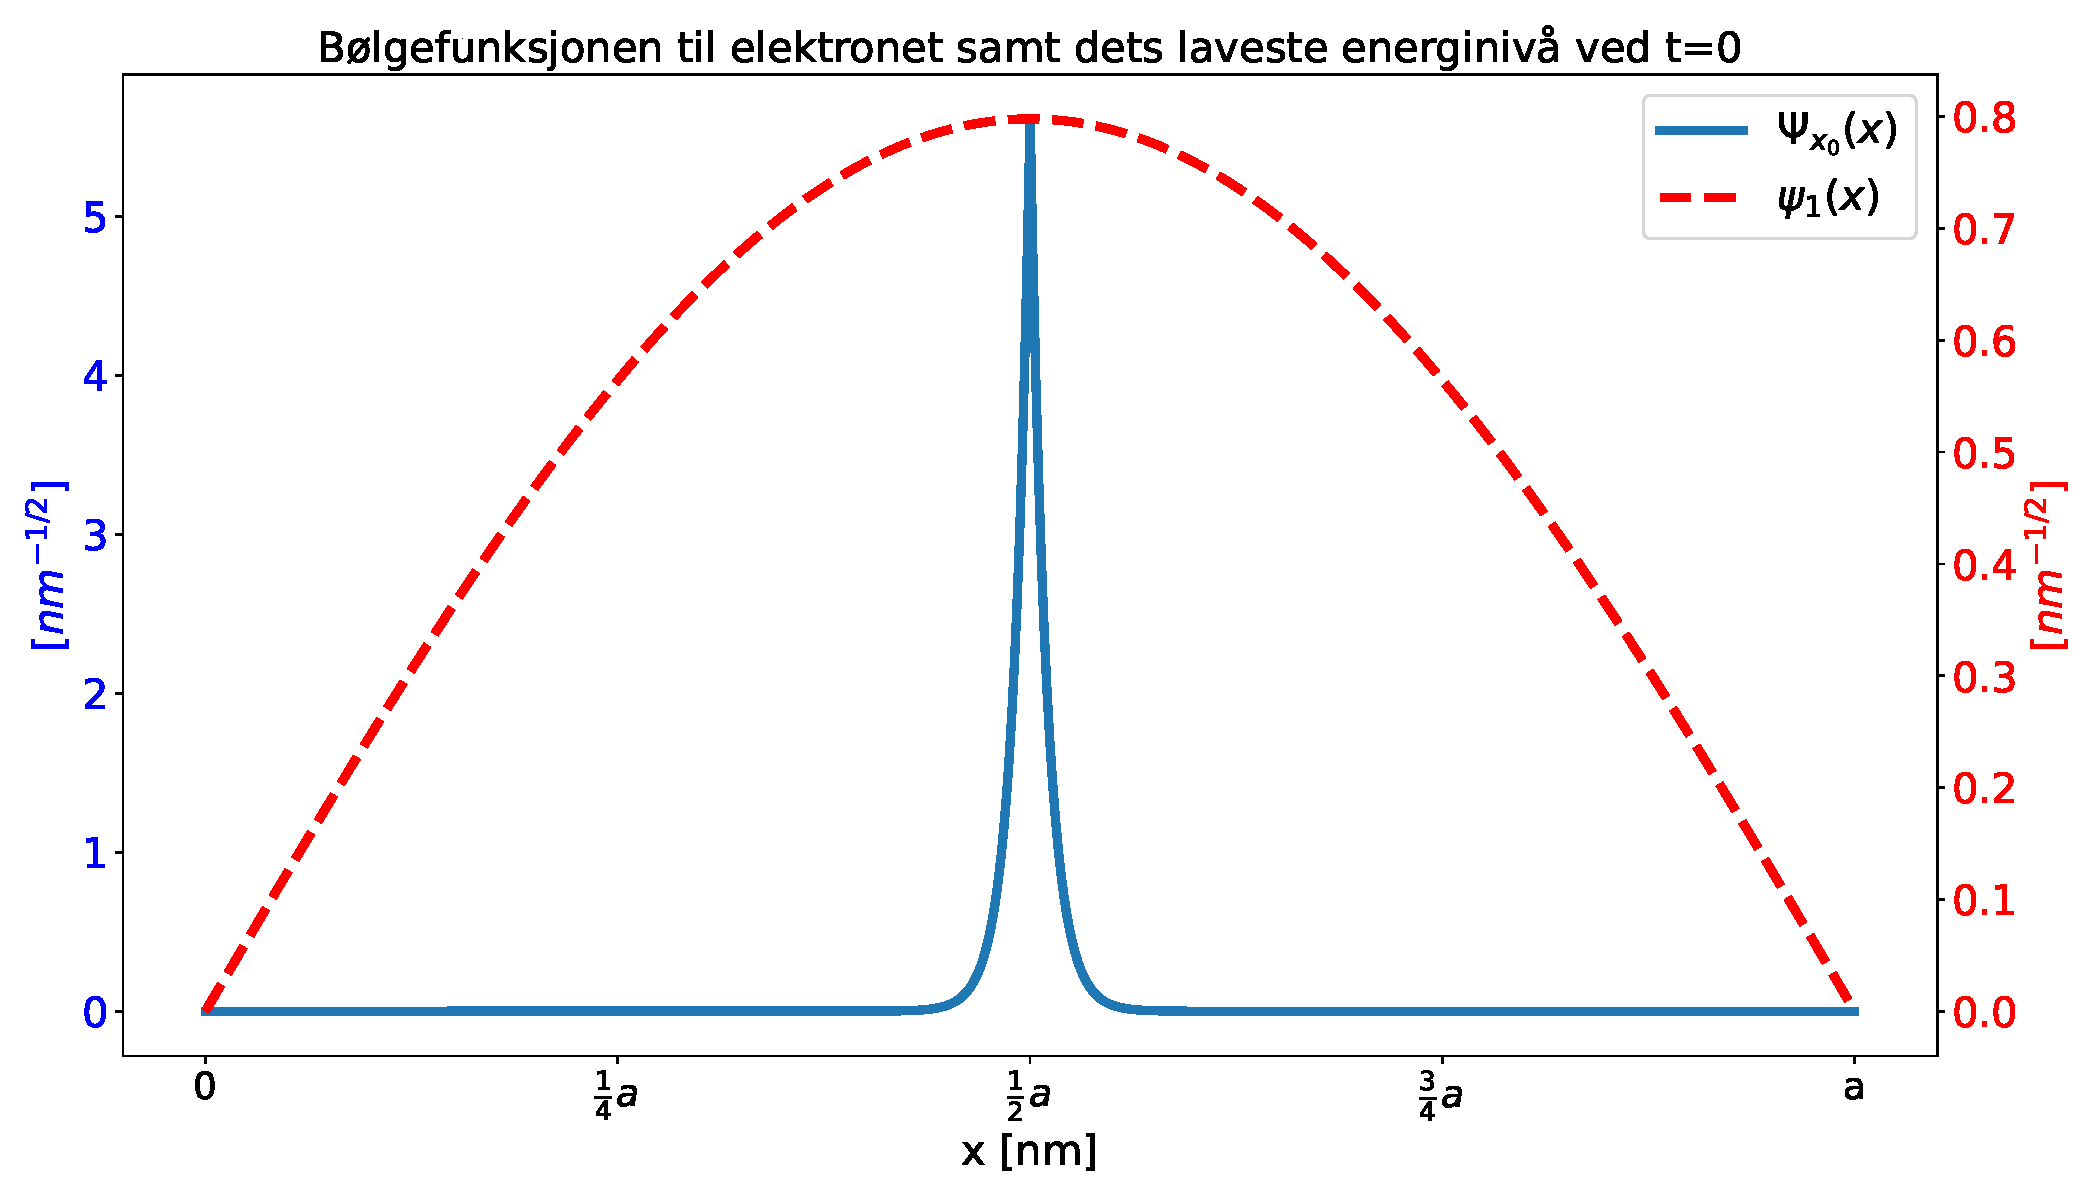
\includegraphics[width = \textwidth]{Midtveis.pdf}
  \caption{Plot av $Ψ_{x_0}(x,0)$ og $ψ_1(x)$}
  \label{fig: 3.e}
\end{figure}


\subsection*{f)}
Sannsynligheten for at en måling av $Ψ_{x_0}(x,0)$ i grunntilstanden for $n=1$ vil være $\left|c_1\right| ^2$. Fra likning 2.40 i Griffiths (versjon 3) har vi et utrykk for $c_n$ som er gitt ved \cref{eq: c_n alt} 
\begin{equation}\label{eq: c_n alt}
c_n = \sqrt{\frac{2}{a}} ∫_{0}^{a} \sin \left(\frac{nπ}{a}x\right)\ Ψ(x,0) \ \mathrm{d}x
\end{equation}
\begin{align}
c_1 &= \sqrt{\frac{2}{a}} ∫_{0}^{a} \sin \left(\frac{1π}{a}x\right)\ Ψ(x,0) \ \mathrm{d}x \\
c_1 &= \sqrt{\frac{2}{aε}} ∫_{0}^{a} \sin \left(x\right)e^{- \left|x - x_0\right| / ε} \ \mathrm{d}x \\
c_1 &= 0.2825 
\end{align}
Sannsynligheten er da $0.2825^2 = 0.0798 ≈ 8.0 \%$. 
Bølgefunksjonen vil etter målingen til grunntilstanden, kollapse til en enkelt verdi. 


\section*{Oppgave 4}
\subsection*{a)}
Vi bruker den rekursive formelen fra likning 2.67 fra Griffiths (versjon 3)

\begin{equation}\label{eq: a rek}
ψ_n = \frac{\sqrt{n}ψ_{n-1}}{\hat{a}_{-}}
\end{equation}
\begin{align}
  ψ_1 &= \frac{\sqrt{1}ψ_{0}}{\hat{a}_{-}} = \frac{ψ_{0}}{\hat{a}_{-}} \label{eq: a_1} \\ 
  ψ_2 &= \frac{\sqrt{2}ψ_{1}}{\hat{a}_{-}} = \frac{\sqrt{2}ψ_0}{\left(\hat{a}_{-}\right)^2} \label{eq: a_2} \\
  ψ_3 &= \frac{\sqrt{3}ψ_{2}}{\hat{a}_{-}} = \frac{\sqrt{6}ψ_0}{\left(\hat{a}_{-}\right)^3} \label{eq: a_3} \\
  ψ_4 &= \frac{\sqrt{4}ψ_{3}}{\hat{a}_{-}} = \frac{\sqrt{24}ψ_0}{\left(\hat{a}_{-}\right)^4} \label{eq: a_4}
\end{align}
Hvis vi stokker om \cref{eq: a_4} får vi 
\[
\left(\hat{a}_{-}\right)^4 ψ_4 = \sqrt{24} ψ_0 = \sqrt{4!}ψ_0
\]
Gjør vi dette for \crefrange{eq: a_1}{eq: a_3} ser vi et klart mønster som vi kan bruke til å finne et eksplisitt formel for $\left(\hat{a}_{-}\right)^{n}ψ_n$.
\begin{equation}\label{eq: psi_n}
\left(\hat{a}_{-}\right)^{n} ψ_n = \sqrt{n!} ψ_0
\end{equation}

\subsection*{b)}
Ettersom $ψ_0$ er det laveste energinivået, vil naturligvis $\left(\hat{a}_{-}\right)ψ_0$ være 0. Videre bruk av operatorene på negative energinivåer (som i utgangspunktet ikke gir mening) vil da naturligvis også gi 0, som vil si at $\left(\hat{a}_{-}\right)^{n}ψ_0 = 0$. Vi ser også at om vi bruker utrykket for $\left(\hat{a}_{-}\right)^{n} ψ_n$ derivert i \cref{eq: psi_n} får vi $\left(\hat{a}_{-}\right)^{n}ψ_0 = \sqrt{0!}ψ_0 = ψ_0$. 


% Setter vi inn utrykket for $ψ_n$ som beskrevet i likning 2.68 i Griffiths (versjon 3) i likningen vi fant i \cref{eq: psi_n}. 
% \begin{align}
% \left(\hat{a}_{-}\right)^{n} ψ_n &= \sqrt{n!} ψ_0 \\
% \left(\hat{a}_{-}\right)^{n} \frac{1}{\sqrt{n!}} \left(\hat{a}_{+}\right)^{n}ψ_0 &= \sqrt{n!} ψ_0 \\
% \left(\hat{a}_{-}\right)^{n} \left(\hat{a}_{+}\right)^{n}ψ_0 &= n! ψ_0 \\
% ψ_0 &= n!ψ_0 \\ 
% \left(\hat{a}_{-}\right)ψ_0 &= n! \left(\hat{a}_{-}\right)ψ_0
% \end{align}
% Ettersom $n! ≠  0$ er den eneste måten likningen kan løses ved følgende: 
% \begin{equation}\label{eq: a_psi_0}
% \left(\hat{a}_{-}\right)ψ_0 = 0
% \end{equation}

% \lstinputlisting[language=Python]{Midtveis.py}

% \begin{lstlisting}[language=Python]
%   import numpy as np 
%   import matplotlib.pyplot as plt
%   import os 
%   filepath = os.path.dirname(__file__)
%   π = np.pi
%   e = np.exp
  
%   # [nm]       [nm]        [nm]     [nm]              [nm]
%   a = π; ε = 0.01*a; x0 = 0.5*a; k = π/a; A = np.sqrt(2/a);
  
%   def ψ(x):
%       return 1/(np.sqrt(ε)) * e(-abs(x-x0)/ε)
  
%   def ψ_1(x):
%       return A*np.sin(1*π/a * x)
  
  
%   x = np.linspace(0,a, 10_000) # [nm]
  
%   fontsize = 20
%   fig, ax1 = plt.subplots(figsize=(14, 8))
%   plot1 = ax1.plot(x, ψ(x), linewidth=4, label = r'$Ψ_{x_0}(x)$')
%   ax1.set_xlabel('x [nm]', fontsize=fontsize)
%   ax1.set_ylabel(r'[$nm^{-1/2}$]', fontsize=fontsize, color='blue')
%   # ax1.yaxis.set_label_coords(-0.2,.45)
%   ax1.set_xticks([0, 0.25*a, 0.5*a, 0.75*a, a], ['0', r'$\frac{1}{4} a$', r'$\frac{1}{2} a$', r'$\frac{3}{4} a$', 'a'], fontsize=fontsize-2)
%   ax1.tick_params(axis='y', labelcolor='blue', labelsize=fontsize)
  
  
%   ax2 = ax1.twinx()
%   plot2 = ax2.plot(x, ψ_1(x), linestyle='--' , color = 'red', linewidth=4, label = r'$ψ_1(x)$')
%   ax2.tick_params(axis='y', labelcolor='red', labelsize=fontsize)
%   ax2.set_ylabel(r'[$nm^{-1/2}$]', fontsize=fontsize, color='red')
%   # ax2.yaxis.set_label_coords(1.25,.475)
  
%   plt.title('Bølgefunksjonen til elektronet samt dets laveste energinivå ved t=0', fontsize=fontsize)
%   plot = plot1 + plot2
%   labels = [l.get_label() for l in plot]
%   plt.legend(plot, labels, fontsize=fontsize)
  
%   plt.tight_layout()
%   plt.savefig(os.path.join(filepath, 'Midtveis.pdf'))
%   plt.show()
% \end{lstlisting}

\end{document}